%This is a Latex file.
\documentclass[12pt]{article}

\usepackage{amsmath, amssymb, amsthm, amscd, amsfonts, dsfont}
\usepackage{mathrsfs}
\usepackage{graphicx}
\usepackage{verbatim}
\usepackage{enumerate}
\usepackage{url,hyperref}
\usepackage{comment}
\usepackage{multicol}
\usepackage{latexsym,fancyhdr}
\usepackage[margin=1in]{geometry}
\usepackage{lastpage} % Required to determine the last page for the footer
\usepackage{tikz}
\usepackage{charter}
\usepackage{bbold}

\parindent 0pt

\pagestyle{fancy} \lhead{\sf MTH 415} \chead{\sf Open Final}
\rhead{\sf Due: Friday 05/15/2020} \lfoot{} \cfoot{} \rfoot{}

\newcommand{\C}{\mathbb{C}}
\newcommand{\R}{\mathbb{R}}
\newcommand{\Q}{\mathbb{Q}}
\newcommand{\Z}{\mathbb{Z}}
\newcommand{\N}{\mathbb{N}}

\renewcommand{\AA}{\mathcal{A}}
\newcommand{\BB}{\mathcal{B}}
\newcommand{\CC}{\mathcal{C}}
\newcommand{\DD}{\mathcal{D}}
\newcommand{\RR}{\mathcal{R}}
\renewcommand{\SS}{\mathcal{S}}
\newcommand{\TT}{\mathcal{T}}

\newcommand{\wts}[1]{\textit{\textcolor{blue}{WTS: #1}}\\}
\newcommand{\pg}{\textit{\textcolor{green}{PG: }}}
\newcommand{\pn}{\textit{\textcolor{yellow}{PN: }}}
\newcommand{\pb}{\textit{\textcolor{orange}{PB: }}}

\newcommand{\1}{^{-1}}

\begin{document}
	\section{Persistence}
	One problem that I really struggled with was Theorem 2.8. Theorem 2.8 states: Let $ A $ be a subset of a topological space $ X $, and let $ A' $ be the set of limit points of $ A $. Then $ Cl(A)=A\cup A' $. What I really struggled with was not the idea itself (which still took some parsing to grok what this really means) but being able to prove this. I distinctly remember three different occasions were I was going through the proof. One was on a long quiz, a second time was with Mason in the Math Lounge, and a third time on the first exam. The first attempt was by all standards a failure, the second time was better but still had several gaps which Mason pointed out and helped fill in, the third time was completely on my own. I was excited when I saw the problem on the exam. I knew the proof, I had worked on it so many times before. This third time was my best, yet it still had a couple of minor details missing. That frustrated me. I couldn't believe that I had gone through this proof so many times and still couldn't remember or have a complete outline of the proof. This was a valuable experience as it showed that often times I assume a greater level of competence than I should. Just because I'm aware of it, does not mean that I *know* it. \\
	\begin{proof}
		\wts{$A\cup A' \subset Cl(A)$}
		Notice, $ A \subset Cl(A) $ by definition of closure. \\
		Suppose $ x\in A' $. Then $ \forall U \subset X $ such that $ x\in U $, we have $ U\cap A \neq \varnothing $. So, we have $ x\in Cl(A) $ by Theorem 2.5. Hence, $ A'\subset Cl(A) $.\\
		Thus, $ A\cup A' \subset Cl(A) $.\\
		\\
		\wts{$Cl(A)\subset A\cup A'$}
		Let $ x\in Cl(A) $. Then, $ x\in A $ or $ x\in Cl(A)-A $.\\
		Case 1: $ x\in A $\\
		Suppose $ x\in A $. Then, $ x\in A\cup A' $\\
		\\
		Case 2: $ x\in Cl(A)-A $.
		Suppose $ x\in Cl(A)-A $.  Then $ \forall U \subset X $ such that $ x\in U $, we have $ U\cap A \neq \varnothing $, by Theorem 2.5. We know that $ x\not\in A $ and so there must exist a point other than $ x $ where $U$ and $A$ intersect. Notice, this is the definition of a limit point. So, $ x $ is a limit point and it follows that $ x\in A' $. \\
		Thus, $x\in A\cup A'$.\\
		\\
		So, for both cases $ x\in A\cup A' $.\\
		Thus, $ Cl(A)\subset A\cup A' $\\
		\\
		Therefore, $ Cl(A)=A\cup A' $
	\end{proof}
	\section{Curiosity}
	I am interested more in how topologies can be applied to network topologies. In computer science, we have the subfield of networking. I think it would be really cool to apply the knowledge in this class on the networking. Once question I would ask is about optimal type of topology. Of course, this would depend on the purposes of the network. By applying a more mathematical view, perhaps we can unveil some changes that can be more efficient or effective. I would also think that determining if two topological networks were topologically equivalent would be useful as well. By creating categories that each network topology falls into, we can easily describe the properties of the network. Another question would be if there is a finite number of network topologies that can be created in the real world with current technologies.
	\section{Imagination}
	In the class I've had to think much more abstractly than usually. From the very beginning every definition has been about some arbitrary space or sets. Sure, we use $ \R^n $ to help visualize but not all situations can be applied through $ \R^n $. I have found after taking this class I am much less concerned about the particulars of a problem, but am more comfortable with thinking in the general. In many proofs, we would draw open neighborhoods around a certain point. At first I wanted to know more about this neighborhood. I wanted to see its exact size and shape. (this probably comes from being used to draw out these shapes in $ \R^2,$ and $ \R^3 $). Now, I realize that these specifics don't really matter. In fact I feel like making these problems more general has made them more powerful. It doesn't matter what situation is presented, I know the results.\\
	\\
	I also found the definition of open sets and closed sets to be very strange at first. I didn't like how open sets were just subsets contained in a set. But over time and usage of these ideas, I felt like I was able to easily grasp what they were and how to use them. It took me even longer with closed sets. I almost always just used that fact that the complement of a closed set is open. And would just work in the open set instead.\\
	\\
	I found connectedness to be an interesting idea as well. At first glance I seemed to understand what being connected was, that is there does not exist a pair of disjoint nonempty open sets whose union is the set. But as we continued on, we learned about path connectedness. And with that we described examples where the space is connected yet not everything is contained in the subset. This lead to spaces being connected, but not path-connected. This took a little bit of processing to understand. I felt like this really helped me to go by the definition described instead of what I felt "had" to be right. 
	\section{Disposition Towards Beauty}
	I think the Chapter 3 with the subspace, product, and quotient topology is beautiful. I think that its amazing that we can take topological spaces and apply operations which are similar to the mathematics we do in $ \R^n $. The product topology is the same concept as multiplying two numbers together. Similarly the quotient space is the same idea as dividing a number by another. To explain this like I was five: You know about numbers yeah? Well, all those numbers represent is a quantity. What if we had these numbers represent something else? This something else would be a topological space. So just like how you can have two numbers and get their product, we can do the same thing with our topological spaces. The really cool part is that these new things are still topological spaces, which parallels with how the product is now a new number. Going with division, we can see that we take parts of a number and get the quotient. We can do the same thing with topological spaces, splitting them into component parts. \\
	\\
	The really beauty of this is cycles and pattern seen throughout mathematics. Humankind is big on finding patterns and making sense of the world. People will find patterns or fixate cause-effect relationships that bear no truth.\\
	\\
	 Even when describing a topological space, the same underlying intuition and structure is layered in even the most theoretical of maths. It makes me wonder if the way we defined these higher level maths is from our intuition with lower level maths or if it's the other way around. That the higher level maths are so structured that even the lower level maths reflect this.

	\section{Creativity}
	I found metrics and metric spaces to be a creative mathematical idea from this class. $ \R^n $ we are most familiar with. It has nice properties and is familiar to most mathematicians. An arbitrary topological space is not so intuitive and easy to visualize. A metric takes the best of $ \R^n $ and defined a way to create more spaces similar to it. A Metric has three (and a half) really nice properties to work with. A metric on a set $ X $ is a function $ d: X\times X \to \R $ with the following properties: Given any points $ x,y,z\in X $,\\
	\\
	(i) $ d(x,y) \geq 0 , d(x,y) = 0 $ if and only if $ x=y $\\
	(ii) $d(x,y)=d(y,x)$\\
	(iii) $d(x,y)+d(y,z) \geq d(x,z)$\\
	\\
	These three properties forms the foundation of a metric space.\\
	A Metric space is Hausdorff. A Hausdorff space has again many more properties that are useful.\\
	When I did a internet search about other properties of Metric Spaces, I came up with a huge list. These properties make talking about and proving statements much easier and intuitive.
	\section{Thinking for Oneself}
	I found problem 7.41 to be interesting. We didn't get to really talk about it this semester, but last year when I took this course we talked about one-point compactification. This is the idea of adding in another point such that the space is now compact. Exercise 7.41 (a) and (b) are about visualizing these one-point compactification.\\
	\\
	(a) Describe and illustrate the result of taking the one-point compactification of the open annulus $S^1\times(0,1)$.\\
	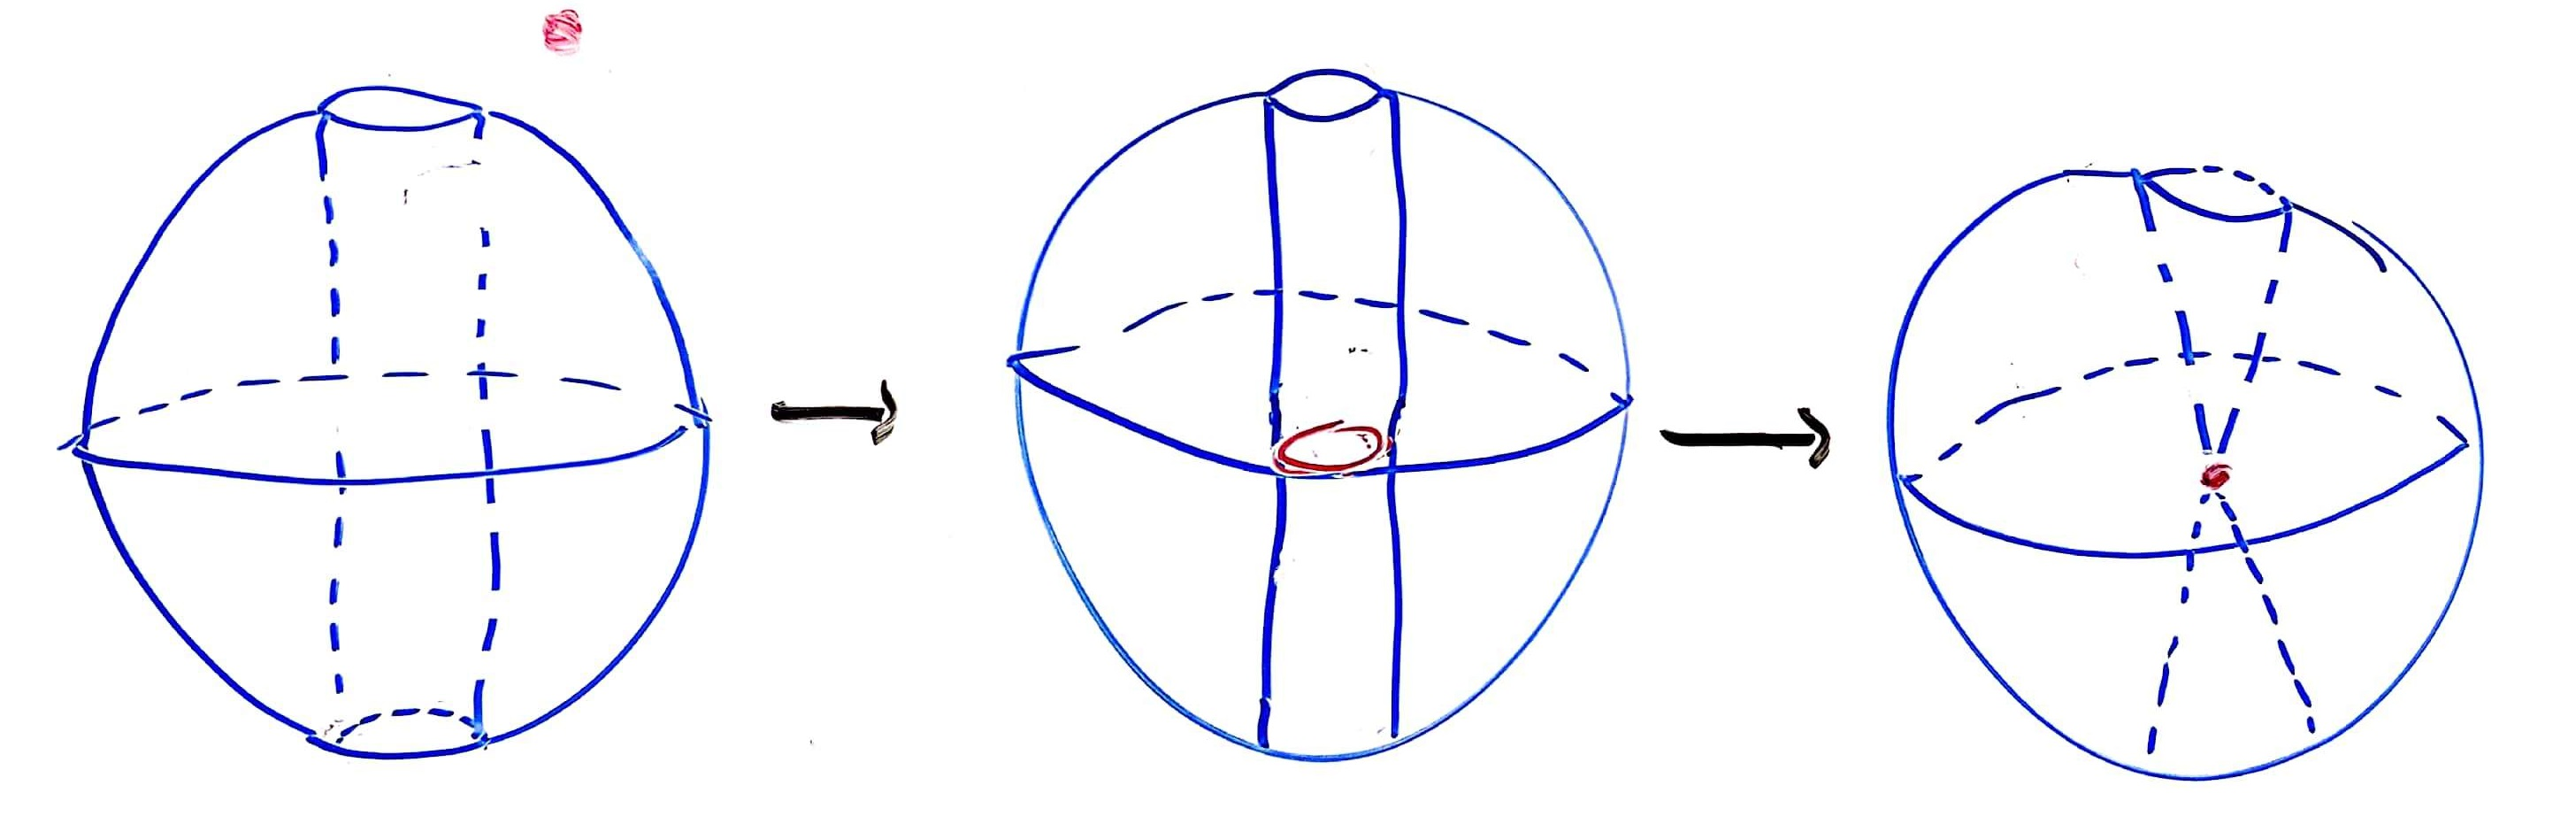
\includegraphics[scale=.28]{7-41a.jpg}
	\\
	(b) An open Mobius band is the space obtained from $[0,1]\times(0,1)$ by gluing the ends as we do with the usual Mobius band.  Describe and illustrate the result of taking the one-point compactification of the open Mobius band. \\
	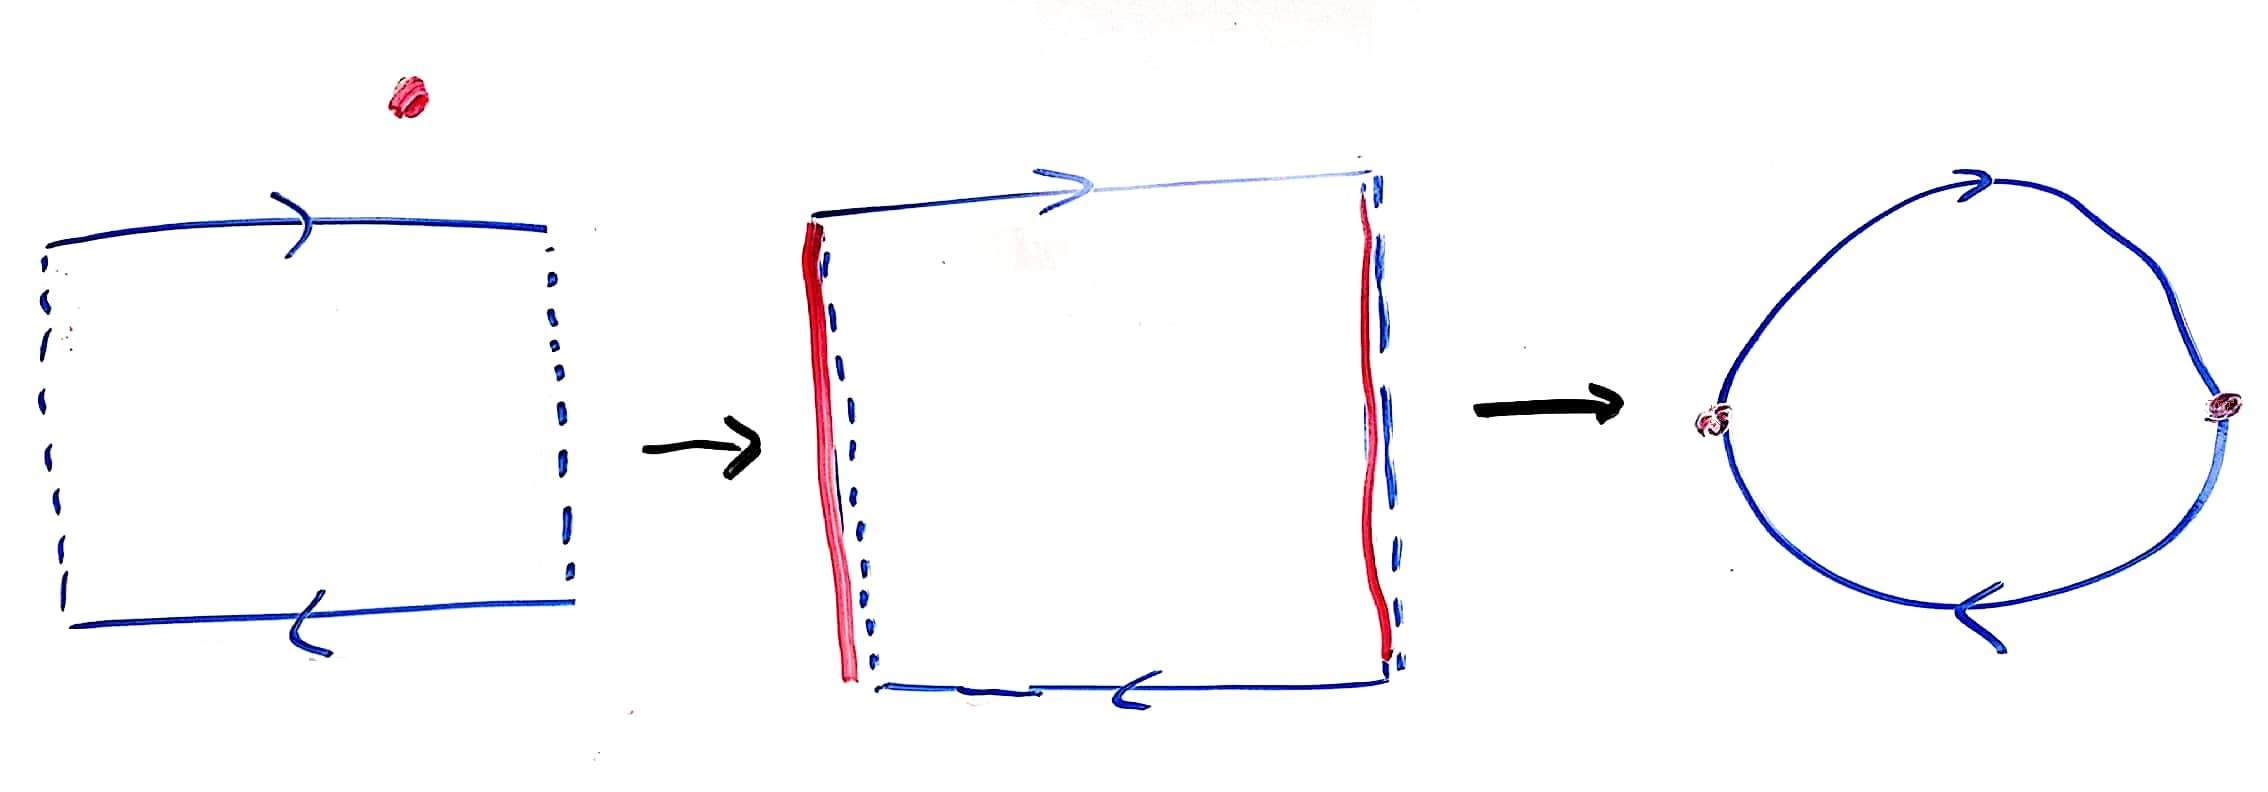
\includegraphics[scale=.3]{7-41b.jpg}
	\\
	 
	
	\section{Talk The Talk, Walk The Walk}
	\begin{enumerate}
		\item Let $ f: X\to Y $ be a map between metric spaces. A subset $ A $ of $ Y $ is connected if and only if $ f\1(Y) $ is connected.\\
		False, a disconnected metric space would map to a single point. This is used to understand metric spaces and connectedness 
		\item Let $ X $ be a topological space and $ A,B\subset X $ be compact. Is $ A\cup B $ compact as well?
		True, by the definition of a compact set. This shows that the student understand the definition of compact.
		\item Let $X$ be a topological space and $ A\subset X $. If $ Int(A)=Cl(A) $, then $ A $ is both open and closed (clopen).
		True, $ Int(A)=A=Cl(A) $. This shows that the student understands interior and closure and well as the independence of being open and closed
		\item $ \R $ with the standard topology is a connected topological space.\\
		True, only $ \varnothing $ and $ \R $ are both open and closed. Shows understanding of connectedness in a familiar topological space.
		\item If $ X $ is a Hausdorff space, then every single-point subset of $ X $ is closed.\\
		True, by theorem 1.9. Shows the student understand some of the properties that Hausdorff spaces have.
		\item Let $ X $ is a Hausdorff space. Then any subspace of $ X $ is Hausdorff.\\
		True, Hausdorff is a topological invariant. Shows understanding of invariants and how they apply to subspaces and homeomorphisms.
		\item Let $X$ be a topological space and $ A\subset X $. If $ A $ is compact in $ X $, then it is closed.\\
		False, consider $ X=[0,1] $ with $ A=\{\frac{1}{2}\} $. Notice, $ A $ is compact but not closed. Tests student of assumptions of compact subsets.
		\item Let $ X $ be a topological space. Then, any path component of $ X $ is closed.\\
		False, consider the Topologist's Since Curve. Shows understanding of path components and path connectedness.
		\item  Let $X$ be a topological space and $ A\subset X $. If $ A $ is not open then it is closed.\\
		False, by definition of open and closed, we cannot say $ A $ is closed based on not being open. Shows understanding that open and closed are not mutually exclusive.
		\item Do the subsets $ \varnothing,\{a\},\{a,b\},\{a,b,c\} $ form a topology?\\
		True, $ \varnothing $ and $ X $ are open sets, the intersection of finitely many open sets is an open set, the union of any collection of open sets is an open set. This shows the understanding of a basic topology.
		
	\end{enumerate}
	
	
	
	
	
	
	
	
	
	
	
	
	
	
	
	
	
	
	
	
	
	
	
\end{document}